\documentclass[10pt]{article}
\usepackage[margin=2cm]{geometry}
\usepackage{amsmath,amssymb}
\usepackage{booktabs}
\usepackage{graphicx}
\usepackage{float}
\usepackage{array,tabularx}
\usepackage[font=small,labelfont=bf]{caption}
\usepackage[compact]{titlesec}
\usepackage{enumitem}
\usepackage{microtype}
\usepackage[hidelinks]{hyperref}
\setlist{itemsep=1pt,topsep=3pt}
\setlength{\parskip}{4pt}
\setlength{\parindent}{0pt}
\graphicspath{{figures/}}
\newcommand{\fig}[1]{Figure~\ref{#1}}
\newcommand{\tab}[1]{Table~\ref{#1}}

\begin{document}
\sloppy

\begin{center}
{\LARGE SuperMimic on Kangaroo, M4: the stability study}\\[4pt]
Why the online loop oscillated, five 12\,h runs on Leonardo to find out, and what we changed. Branch
\texttt{omm/supermimic} of pal\_mjlab, 26 October 2026.
\end{center}

\section*{Summary}

\begin{itemize}
  \item \textbf{The oscillation came from an early critic blow-up, and two small changes prevent it.}
  In the first 2000 iterations a run either blew up its critic (value down to $-175$ to $-396$, loss up
  to $10^8$) or did not. The two runs whose policy uses that critic and blew it up (baseline, A6) kept
  spiking afterwards. No run that avoided the blow-up ever spiked. A1 blew up its critic too, but its
  policy does not use it, and it stayed stable.
  \item \textbf{B, A2$'$ and A5 trained without a single collapse} in 12\,h: no failure spike or
  critic-loss burst at any iteration, and no collapse at any checkpoint benchmarked so far (every 2000
  iterations; the odd thousands follow). Their benchmark rises
  steadily to tracking return 0.89 with 2--5 failed clips (of 1296). That beats the old baseline's best
  checkpoint in its full 24\,h run (0.872), and it gets there in about 20,000 iterations. The baseline
  collapsed 3 times over the same iterations.
  \item \textbf{B is the plain algorithm with another seed}: it avoided the blow-up by chance. A2$'$
  (failure head on the rule's two errors) and A5 (critic loss weighted by survival) avoid it by design.
  A2$'$ is also the fastest: 4 failures after 2000 iterations, against 48--49.
  \item \textbf{A1 (no critic) is stable but worse}: 16--23 failures at its best and last checkpoints,
  against 2--5. Without the blow-up the critic is not what makes training unstable, and it helps
  tracking.
  \item \textbf{A6 (no privileged critic inputs) does not help}: it blew up early and spiked like the
  baseline (same seed), and reached only 0.711 by iteration 20,000. Stopped at 6\,h.
  \item \textbf{Adopted: A2$'$ and A5 together} as the default (D39), now in the 24\,h \texttt{full}
  and \texttt{dev} runs. Both are stable at about iteration 18,000 so far.
  \item One run per configuration. The changes are large and systematic, but the exact numbers of a
  single run carry seed noise.
\end{itemize}

\section{The question}

SuperMimic's online loop oscillated on \texttt{dev}, locally (bf16, replay 500) and on the cluster with
the paper's settings (TF32, replay 1000; \texttt{cluster\_report.pdf}). The policy repeatedly collapsed
from a few failures to most clips failing, and recovered. Before the runs, a diagnostic on the old
checkpoints (\texttt{scripts/supermimic/reward\_extremes.py}) separated two mechanisms:
\begin{enumerate}
  \item \textbf{The main collapses: the critic goes wrong on live states.} Between the checkpoint before
  a collapse and the collapse checkpoint, the critic's error on imagined steps before any predicted fall
  grows 40--150$\times$. The critic overestimates where the robot is still up, and the policy follows its
  gradient (about 70\% of the policy's objective is the critic's value at step 32).
  \item \textbf{A late burst: post-fall extrapolation.} After an imagined fall the world model is
  outside its data and its predicted joints run away. The joint-limit penalty, linear and unbounded,
  reaches $-10^6$ per step. The policy's objective weights those steps by the survival $\hat c_t\approx0$,
  but the paper's critic loss (Eq.~3) does not, so a few such rollouts dominate it (loss up to
  $10^{14}$).
\end{enumerate}

\section{The runs}

One change per run against the cluster baseline (seed 42), all from one commit, 12\,h on one A100 each,
with the paper's settings and compiled imagination (D37). Every checkpoint (every 1000 iterations) is
benchmarked on the same 1296 \texttt{dev} clips as all earlier runs, every clip once from its first
frame.

\begin{table}[H]
\centering\small
\begin{tabularx}{\textwidth}{@{}l>{\raggedright\arraybackslash}X>{\raggedright\arraybackslash}X@{}}\toprule
run & change & what it tests \\\midrule
B & none, seed 43 & run-to-run variance \\
A1 & no critic ($H = 32$) & do the collapses need the critic? (also the paper's Fig.~4b cell) \\
A2$'$ & failure head on the rule's two errors (root height, gravity-$z$; 64$\times$64) instead of
256$\times$256 on the full state, as SuperMimic-Reproduced & does the policy exploit the learned head? \\
A5 & critic loss weighted by $\hat c_t$ (a deviation from Eq.~3) & does post-fall data poison the
critic? \\
A6 & critic without our privileged inputs (root-pose error, time left) & do our critic additions (D7, D22)
mislead it? Stopped at 6\,h. \\
\bottomrule
\end{tabularx}
\end{table}

\section{Training signals}

\begin{figure}[H]
\centering
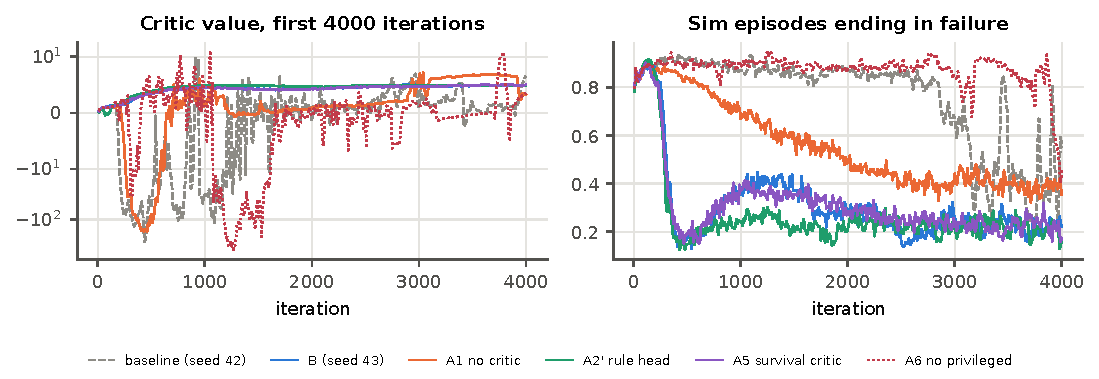
\includegraphics[width=\textwidth]{stability_early.pdf}
\caption{The first 4000 iterations. Left: the critic's value of the imagined start states (symmetric
log scale). Right: the share of simulator episodes ending in a failure.}
\label{fig:early}
\end{figure}

\textbf{Early on, the runs split in two} (\fig{fig:early}).
\begin{itemize}
  \item \textbf{A critic blow-up in the first 2000 iterations} hit the baseline, A6 and A1. Their
  critic's value fell to $-277$, $-396$ and $-175$, and its loss reached $10^6$--$10^8$. These runs took
  off late: the share of failing episodes first dropped below 50\% at iterations 3160, 3980 and 1970.
  A1's critic is trained but not used by its policy, which is why it recovered sooner.
  \item \textbf{B, A2$'$ and A5 never had one.} Their value stayed between 0 and 5, and they took off at
  iterations 310, 290 and 300.
  \item \textbf{Likely mechanism.} At the start, the 256$\times$256 learned head ranks failures worse than
  chance (AUC about 0.4). So imagined falls keep their survival weight, and the exploding post-fall
  penalties flood both the policy's objective and the critic's targets.
  \begin{itemize}
    \item A2$'$'s two-feature head learns failure almost at once, so falls are cut off.
    \item A5 keeps post-fall steps out of the critic's fit.
    \item B avoided it by chance; its seed alone made the difference.
  \end{itemize}
\end{itemize}

\textbf{Afterwards} (\fig{fig:training}, up to iteration 35,520, the shortest run):
\begin{itemize}
  \item \textbf{B, A1, A2$'$ and A5 had no failure spike and no critic-loss burst at all.} Their
  critic loss stayed near $10^{-2}$ and their policy gradient near 0.5 throughout. Imagination tracked
  the simulator at a correlation of 0.99 or more at every check.
  \item \textbf{The baseline} had 7.2 failure spikes per 10,000 iterations and 15 critic-loss bursts over
  the same range. \textbf{A6} had 5.8 spikes per 10,000 before it was stopped. Both had checks where
  imagination and simulator disagreed (correlation down to 0.15 and 0.66).
  \item \textbf{A1 is calm but tracks a little worse.} Over the last 10,000 iterations, 29\% of its
  training episodes end in a failure, against 20--21\% for the others; its 32-step failure rate in the
  simulator is 3.5\%, against 1.1--1.6\%. Without the critic the policy is more myopic.
  \item \textbf{Extreme imagined rewards still occur} in every variant, because the post-fall
  extrapolation is untouched (iterations with a reward below $-1$: A5 14, B 25, A2$'$ 169, A1 676, A6 560).
  In the stable runs they no longer reach the critic in force: A5 down-weights them, and A2$'$'s sharp
  head stops them from propagating backward through the $\lambda$-returns.
\end{itemize}

\begin{figure}[H]
\centering
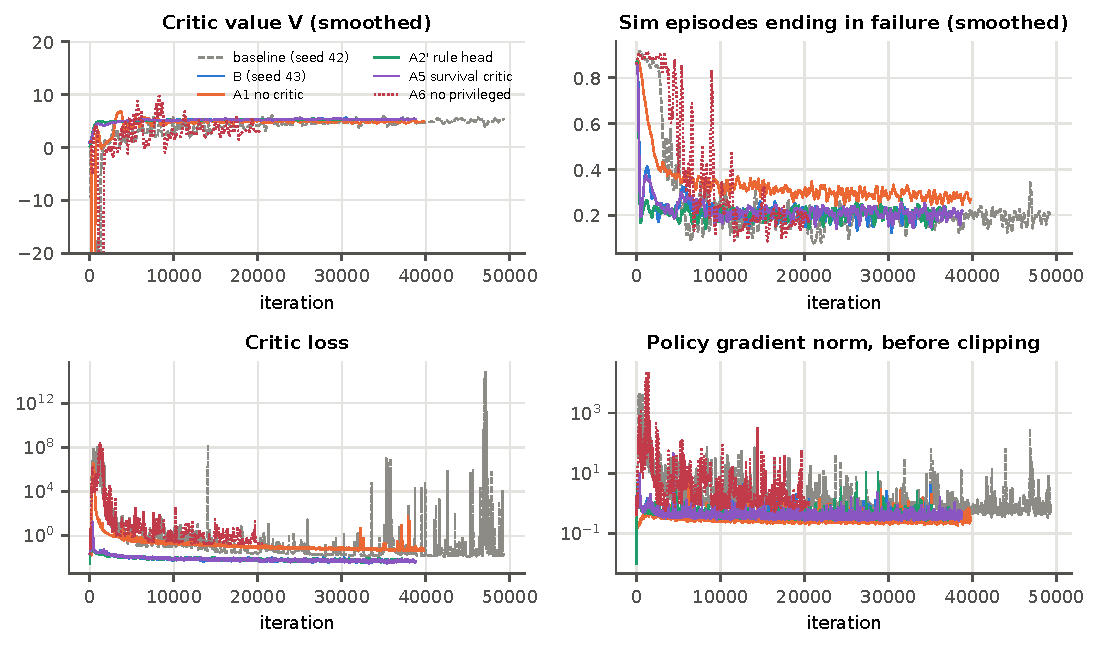
\includegraphics[width=\textwidth]{stability_training.pdf}
\caption{All iterations. Critic value and the share of failing episodes are moving averages; the critic
loss and the policy gradient norm (before clipping) are raw.}
\label{fig:training}
\end{figure}

\section{Benchmark}

\begin{figure}[H]
\centering
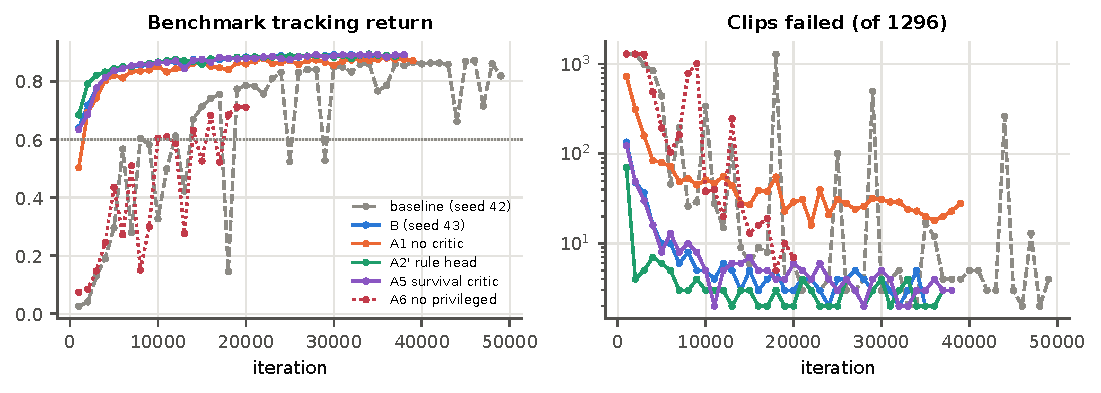
\includegraphics[width=\textwidth]{stability_benchmark.pdf}
\caption{The benchmark of every checkpoint (1296 \texttt{dev} clips, each once from its first frame).
The failure axis is logarithmic; zero failures are drawn at 1. The
baseline is shown over its whole 24\,h run; the table cuts every run at iteration 35,520.}
\label{fig:benchmark}
\end{figure}

\begin{table}[H]
\centering\small
\caption{Per run, up to the shortest run's last iteration (A6: until it was stopped). Early min $V$: the
critic's lowest value in the first 3000 iterations. Take-off: the first checkpoint at PPO-Sim's local
12\,h tracking return (0.742). Best and last: failures / tracking return. Collapses: checkpoints with
tracking return below 0.6 after take-off. Spikes: onsets of training-episode failure spikes after
iteration 5000. Critic bursts: logged critic losses above $10^3$.}
\label{tab:summary}
\resizebox{\textwidth}{!}{\begin{tabular}{lrrrrrrrr}\toprule
run & up to & early min V & take-off & best & last & collapses & spikes/10k & critic bursts \\\midrule
baseline (seed 42) & 35,520 & -277.0 & 17,000 & 2 / 0.861 & 17 / 0.767 & 3 of 19 & 7.2 & 15 \\
B (seed 43) & 35,520 & 0.3 & 4,000 & 4 / 0.892 & 5 / 0.885 & 0 of 16 & 0.0 & 0 \\
A1 no critic & 35,520 & -175.3 & 4,000 & 16 / 0.878 & 23 / 0.871 & 0 of 16 & 0.0 & 0 \\
A2' rule head & 35,520 & -0.4 & 2,000 & 2 / 0.894 & 2 / 0.894 & 0 of 17 & 0.0 & 0 \\
A5 survival critic & 35,520 & 0.3 & 4,000 & 2 / 0.892 & 3 / 0.891 & 0 of 16 & 0.0 & 0 \\
A6 no privileged & 20,530 & -395.8 & -- & 7 / 0.711 & 7 / 0.711 & 0 of 0 & 5.8 & 1 \\
\bottomrule\end{tabular}
}
\end{table}

\begin{itemize}
  \item \textbf{No collapse in B, A2$'$, A5 or A1.} Between benchmarked checkpoints, the tracking return
  never drops by more than 0.02. Over the same 35,520 iterations, the baseline collapsed 3 times: 1287 failures at 18,000, and
  checkpoints below 0.6 at 25,000 and 29,000.
  \item \textbf{Fast take-off.} B, A2$'$ and A5 pass PPO-Sim's local 12\,h level (0.742) by iteration
  4000, A2$'$ by 2000. The baseline needed 17,000.
  \item \textbf{Better at the end.} B, A2$'$ and A5 reach 0.885--0.894 with 2--5 failures. The
  baseline's best, over its whole 24\,h run, was 0.872 with 2 failures (iteration 46,000).
  \item \textbf{A2$'$ leads early}: 4 failures at iteration 2000 and 3 by 8000. B and A5 get down to
  about 5 failures only by iteration 10,000.
  \item \textbf{A1} improves steadily but stays at 16--84 failures after take-off (tracking return up
  to 0.880). Without the critic's value beyond 32 steps, the policy is more myopic.
  \item \textbf{A6} never reaches 0.742 before it was stopped: 7 failures, tracking return 0.711 at
  20,000.
\end{itemize}

\textbf{Caveat: the checkpoints at odd thousands are still being benchmarked.} Two of the baseline's
collapses (25,000 and 29,000) showed only at odd checkpoints, so ``no collapse'' becomes final only once
they are in. The training signals, which cover every iteration, already show no failure spike and no
critic-loss burst in these runs.

\section{What this means}

\begin{enumerate}
  \item \textbf{The instability was a consequence of the early blow-up, not a property of the
  algorithm.} The same code, with nothing changed (B), trained stably when it happened to avoid the
  blow-up. The runs that went through one (baseline, A6) kept spiking for tens of thousands of
  iterations. The damage persists, for example in the critic's weights or in Adam's moment estimates;
  we did not isolate which.
  \item \textbf{The cause of the blow-up is the post-fall extrapolation, unweighted.} Early, the learned
  head misses falls, so exploding post-fall penalties enter the policy's objective and every critic
  target. A2$'$ removes the first route by making the survival weights right from the start. A5 removes
  the second by keeping post-fall steps out of the critic's fit.
  \item \textbf{Removing our privileged critic inputs does not help.} A6 (root-pose error and time
  left removed) blew up and spiked like the baseline, which has the same seed. Whether D7 and D22 help on
  their own is not settled; they stay.
  \item \textbf{The critic helps tracking.} Without it (A1) training is stable, but the policy fails
  several times more clips (16--23 against 2--5 at the end).
\end{enumerate}

\section{Also learned along the way}

\begin{itemize}
  \item \textbf{The code is not what made the new runs calm.} One update, computed by the old and the
  new code on identical inputs, agrees to $10^{-6}$ in FP32. In TF32, rounding alone, amplified through
  the 32-step backward pass, moves the actor gradient by 3--12\%. That changes which chaotic trajectory
  a run follows, as a seed does, but not its expected behavior.
  \item \textbf{Speed.} Compiling the imagination step and the world-model loss (D37) brings an A100
  iteration from 1.78\,s to about 1.1\,s. CUDA graphs on top (D41) measured 2.8$\times$ on the policy
  update in isolation, but hung in the training loop. They are not used.
  \item \textbf{The return-based sampler concentrates.} Once the policy is good, about half of the starts
  go to about 1\% of the bins. One clip (\texttt{jog\_butt\_kick\_R\_loop\_002}) gets 7--42\% of all
  starts. This is not a collapse trigger, but it heavily skews the training data.
  \item \textbf{Two infeasible clips} sink 6--23\,cm below the ground and fail in every good policy. They
  were removed from the dataset (D40); this report's benchmarks still use the 1296-clip \texttt{dev}.
  \item \textbf{The local GPU queue preempted itself.} The queue daemon's game check matched the
  \texttt{pgrep} of concurrent \texttt{gpuq} status calls, so polling the queue killed running jobs
  (reported, not fixed here).
\end{itemize}

\section{Decisions}

\begin{itemize}
  \item \textbf{D39, adopted:} the failure head on the rule's two errors (64$\times$64) and the
  survival-weighted critic loss are the default. A2$'$ and A5 each prevent the blow-up alone; together
  they cover both routes. The paper's variants stay available by flag.
  \item \textbf{D40:} the two infeasible clips are out of the dataset.
  \item \textbf{D37:} compiled imagination, about 1.1\,s per iteration on an A100. \textbf{D41:} CUDA
  graphs not used until they work in the training loop.
  \item \textbf{Running now} (\texttt{docs/supermimic/m5/runs.md}): \texttt{full} (124,077 clips) and
  \texttt{dev} (1294 clips), 24\,h each with these defaults.
  \item \textbf{Open:}
  \begin{itemize}
    \item benchmark the 24\,h runs;
    \item a second seed of the combined default, to put a number on run-to-run noise;
    \item the sampler's concentration on a few clips;
    \item CUDA graphs in the training loop.
  \end{itemize}
\end{itemize}

\appendix
\section{Reproduction}

\begin{footnotesize}
\begin{verbatim}
# runs (Leonardo, lazyhpc run folders 20261025-153632_<job>_5eb28ab), one flag each, e.g.
python -m pal_mjlab.scripts.supermimic.train Mjlab-SuperMimic-Flat-Pal-Kangaroo-Grippers-ArmWaist1Hz \
  --env.commands.motion.dataset <dataset> --env.commands.motion.subset dev \
  --agent.experiment-name supermimic_stability --agent.run-name A5-survival \
  --agent.algorithm.critic.survival-weighted True
# diagnostic of old checkpoints; benchmark on the 1296-clip dev
python -m pal_mjlab.scripts.supermimic.reward_extremes --task <task> --checkpoints <run>/model_N.pt --out-dir <dir>
python -m pal_mjlab.scripts.supermimic.eval --task <task> --library <dataset>/libraries_archive/dev_1296 \
  --checkpoints <run>/model_*.pt --out-dir logs/supermimic_eval/stability_<run>
# figures, tables, this report
python docs/supermimic/m4/make_stability_figures.py && (cd docs/supermimic/m4 && latexmk -pdf stability_report.tex)
\end{verbatim}
\end{footnotesize}

\end{document}
